	\documentclass[reprint,english,notitlepage,nofootinbib]{revtex4-1}  % defines the basic parameters of the document
% if you want a single-column, remove reprint

% allows special characters (including æøå)
\usepackage[utf8]{inputenc}
% \usepackage [norsk]{babel} %if you write norwegian
\usepackage[english]{babel}  %if you write english


\usepackage{makecell}       %denne gjør at man kan ha nye linjer

\usepackage{physics,amssymb}  % mathematical symbols (physics imports amsmath)
\usepackage{graphicx}         % include graphics such as plots
\usepackage{xcolor}           % set colors
\usepackage{hyperref}         % automagic cross-referencing (this is GODLIKE)
\usepackage{tikz}             % draw figures manually
\usepackage{listings}         % display code
\usepackage{subfigure}        % imports a lot of cool and useful figure commands

% defines the color of hyperref objects
% Blending two colors:  blue!80!black  =  80% blue and 20% black
\hypersetup{ % this is just my personal choice, feel free to change things
    colorlinks,
    linkcolor={red!50!black},
    citecolor={blue!50!black},
    urlcolor={blue!80!black}}

%% Defines the style of the programming listing
%% This is actually my personal template, go ahead and change stuff if you want
\lstset{ %
	inputpath=,
	backgroundcolor=\color{white!88!black},
	basicstyle={\ttfamily\scriptsize},
	commentstyle=\color{magenta},
	language=Python,
	morekeywords={True,False},
	tabsize=4,
	stringstyle=\color{green!55!black},
	frame=single,
	keywordstyle=\color{blue},
	showstringspaces=false,
	columns=fullflexible,
	keepspaces=true}


\begin{document}


\title{FYS3150 - Project 2}
\date{\today}
\author{Vegard Falmår and Sigurd Sørlie Rustad}
\affiliation{Universitetet i Oslo}

\email{vegardfa@uio.no}
\email{sigurdsr@gmail.com}
\newpage

\begin{abstract}

	
Many potentials can be approximated, at least in some intervals, with a HO (harmonic oscillator) potential. In this report we study one and two particles bounded in a such potential, while they interact with a electric force. When you try to solve Schrodinger's equation for both situations you end up with a eigenvalue/-vector problem. We solved this using Jacobi's rotation algorithm. To make sure the algorithm worked properly we tested it using unit-tests and applying it to problems with analytical solutions. For one particle we found the lowest eigenvalue $\lambda = 3.000$. This is close to the analytical term of $\lambda_{ana} = 3$. For two particles we got the eigenvalues (for lowest energy state) $\lambda = 0.841, 2.231, 4.058, 17.444$ with the corresponding frequencies $\omega_r = 0.01, 0.5, 1, 5$. Because eigenvalue correspond to energy, this means that the energy gets higher with larger frequency $\omega_r$. After plotting the eigenvectors we deduced that for higher frequencies orbits become smaller and relative position sharper.
\end{abstract}
\maketitle


\section{Introduction}

The harmonic oscillator (HO) potential appears in many areas within quantum physics. This is because many potentials can be approximated, at least in some intervals, with a HO potential. The most famous example of this might be the model for a hydrogen atom, where the electron is bound to the proton by a HO potential. That is why, in this report, we are going to study both one and multiple electrons in a HO potential. We are also going to account for electrical forces between the particles.

When we try to solve Schrodinger's equation for both one and two particles, we end up with a eigenvalue problem (see theory section). This can be represented with a linear set of equations written on matrix-form (a derivation can be found in our project 1\footnote{github.com/sigurdru/FYS3150/blob/master/Project1/tex/Project1.pdf}). Using Jacobi's rotation algorithm, also described in the theory section, we can diagonalize the matrix to find these eigenvalues and eigenvectors. Then plot the results, comparing them to experimental values.

When implementing algorithms it is important to test your code and make sure it performs as expected. Therefore we perform unit-tests to make sure sections of our program works as expected. We also test the code with a test scenario (buckling beam), which have analytical eigenvalues and eigenvectors. The testing is described in the appendix (section \ref{appendix}).

For our studies we have used c++ for heavy computation, python for visualization and bash for automation. All the code along with instructions on how to run it, can be cloned from our GitHub repository here\footnote{github.com/sigurdru/FYS3150/tree/master/Project2}.


\section{Theory}

\subsection{Unitary transformation}
The transposed of a unitary matrix ($U$) is its inverse.
\begin{equation*}
	U^T = U^{-1}
\end{equation*}
From this we can prove that a unitary transformation preserves the orthonormality of vectors. Consider the set of orthonormal vectors $\{ \mathbf{v}_i \}_i$ and the unitary transformation $\{ U\mathbf{v}_i \}_i = \{ \mathbf{w}_i \}_i$.
\begin{align*}
	\mathbf{w}_i^T\mathbf{w}_j &= (U\mathbf{v}_i)^TU\mathbf{v}_j \\
	&= \mathbf{v}_i^TU^TU\mathbf{v}_j = \mathbf{v}_i^T\mathbf{v}_j \\
	&= \delta_{i,j}
\end{align*}
We notice that orthonormality is perserved.

\subsection{Jacobi's rotation algorithm}
Jacobi's rotation algorithm uses unitary transformations to diagonalize a matrix. A detailed description of the algorithm can be found here \citep{lecnotes}, however we will describe it briefly. In order to diagonalize a given matrix $A$, as mentioned over, we perform a series of unitary transformations.
\begin{equation*}
	B = U_n^T U_{n-1}^T ... U_0^T A U_0 ... U_{n-1}U_n
\end{equation*}
Here $U_i$ are the unitary matrices and $B$ the resulting diagonal matrix. An example of how $U_i$ can look is given under.
\begin{equation*}
	  \begin{bmatrix}
	1  & 0 & ...  & 0 & 0 & ... & 0 & 0 \\
	0 & 1  & ... & 0 & 0 & ... & 0 & 0 \\
	...  & ... & ... & ... & ... & ... & 0 & ... \\
	0  & 0 & ... & \cos \theta & 0 & ... & 0 & \sin \theta \\
	0  & 0 & ... & 0 & 1 & ... & 0 & 0 \\
	...  & ...& ...  &... & ...   & ... &1 &...  \\
	0  & 0& ...  & -\sin \theta &0 & ... &0 &\cos \theta  \\
	\end{bmatrix}
\end{equation*}
The geometric interpretation is that $U_i$ performs a rotation on $T$ in order to zero out non-diagonal elements. It turns out that the fastest way to do this, is to zero out the largest non-diagonal matrix-element. First We define:
\begin{equation*}
	\cot(\theta) = \tau = \frac{a_{ll} - a_{kk}}{2a_{kl}},
\end{equation*}
Where $a_{kl}$ is the largest non-diagonal element in $A$. Now to shorten notation we use $\tan(\theta) = t = s/c$, where $s = \sin(\theta) \wedge c = \cos(\theta)$. By defining $\theta$ such that $a_{kl}$ becomes zero we get the quadratic equation
\begin{equation*}
	t^2 + 2\tau t -1 = 0 \implies t = -\tau \pm \sqrt{1+\tau^2},
\end{equation*}
and can also obtain $c$ and $s$
\begin{equation*}
	c = \frac{1}{1+t^2} \wedge s = tc.
\end{equation*}
The actual transformation is defined by the set of equations
\begin{align}
\begin{split}
	b_{ik} &= a_{ik}c - a_{il}s, i \neq k, i \neq l \\
	b_{il} &= a_{il}c + a_{ik}s, i \neq k, i \neq l \\
	b_{kk} &= a_{kk}c^2 - 2a_{kl}cs + a_{ll}s^2 \\
	b_{ll} &= a_{ll}c^2 + 2a_{kl}cs + a_{kk}s^2 \\
	b_{kl} &= (a_{kk} - a_{ll} )cs + a_{kl}(c^2 - s^2)
	\label{eq:jacobi}
\end{split}
\end{align}
Where $b_{ij}$ are elements in $B$, again see \citep{lecnotes} for a more detailed description of the algorithm. The last line in \ref{eq:jacobi} effectively sets the element to zero. By doing this manually, we can safely cut the number of FLOPS.

An interesting question is; what happens to the eigenvectors and eigenvalues? Because $B$ is diagonal the eigenvectors are just vectors with a $1$ in one element and $0$ everywhere else. We consider an arbitrary eigenvector $\mathbf{v}$ and eigenvalue $\lambda$ that satisfy
\begin{equation*}
	B\mathbf{v} = \lambda \mathbf{v} .
\end{equation*}
Applying the unitary transforms we get
\begin{align*}
	B\mathbf{v} &= U_n^T U_{n-1}^T ... U_0^T A U_0 ... U_{n-1}U_n \mathbf{v} \\
	&= \lambda \mathbf{v} \\
 \end{align*}
We notice that this is true if
\begin{equation}
	\mathbf{v'} = U_0 ... U_{n-1}U_n \mathbf{v}
	\label{eq:vmark}
\end{equation}
is an eigenvector with eigenvalue $\lambda$ that satisfy
\begin{equation*}
	A \mathbf{v}' = \lambda \mathbf{v}'
\end{equation*}
Therefore, if you have the eigenvector $\mathbf{v}$ and matrices $U_i$ you can find $\mathbf{v}'$ with equation (\ref{eq:vmark}).


\subsection{Electrons in a harmonic oscillator potential}

It turns out that if you try to solve Schrodinger's equation you end up with a eigenvalue problem. We will derive the math here, but everything is taken from here \citep{oppgavetekst}. First we consider the Schrodinger's equation for one electron. Because of spherical symmetry we only need to look at the radial part.
\begin{equation}
	-\frac{\hbar^2}{2m}\bigg(\frac{1}{r^2}\frac{d}{dr}r^2\frac{d}{dr}-\frac{l(l+1)}{r^2}\bigg)R(r) + V(r) R(r) = ER(r)
	\label{eq:SE}
\end{equation}
Where $R(r)$ is the radial wave equation, $V(r)$ the potential, $l$ orbital momentum and $r$ distance from the origin. Now because we only have one electron we end up with the HO potential $V(r) = (1/2)kr^2$. Substituting $R(r) = (1/r)u(r)$ and $\rho = (1/\alpha)r$ (where $\alpha$ is a constant with dimension length) we obtain
\begin{equation*}
	-\frac{\hbar^2}{2m\alpha^2}\frac{d^2}{d\rho^2}u(\rho) + \left(V(\rho) + \frac{l(l+1)}{\rho^2}\frac{\hbar^2}{2m\alpha^2}\right)u(\rho) = Eu(\rho).
\end{equation*}
Setting the orbital momentum $l=0$, inserting $V(\rho) = (1/2)k\alpha^2\rho^2$ and defining
\begin{equation*}
	\alpha \equiv \left(\frac{\hbar^2}{mk}\right)^{1/4} \wedge \lambda \equiv \frac{2m\alpha^2}{\hbar}E
\end{equation*}
Schrodinger's equation can then be described by the simple equation (\ref{eq:SE1}).
\begin{equation}
	-\frac{d^2}{d\rho^2}u(\rho)+\rho^2u(\rho) = \lambda u(\rho)
	\label{eq:SE1}
\end{equation}
Now we can expand our model to two particles with Coulomb potential between them. First introducing the relative position $\mathbf{r}$ and center-of-mass coordinate $\mathbf{R}$
\begin{equation*}
	\mathbf{r} = \mathbf{r_1} - \mathbf{r_2} \wedge \mathbf{R} = \frac{1}{2(\mathbf{r_1}+\mathbf{r_2})}.
\end{equation*}
Where $\mathbf{r_1}$ and $\mathbf{r_2}$ are the particles positions.Then the radial Schrodinger's becomes
\begin{equation*}
	\left(  -\frac{\hbar^2}{m} \frac{d^2}{dr^2} -\frac{\hbar^2}{4 m} \frac{d^2}{dR^2}+ \frac{1}{4} k r^2+  kR^2\right)u(r,R)  = E^{(2)} u(r,R).
\end{equation*}
$E^{(2)}$ denotes the fact that we are looking at the total energy of two particles. From an ansatz for the wave equation, we can perform separation of variable on $r$ and $R$.
\begin{equation*}
	u(r, R) = \psi(r)\phi(R) \wedge E^{(2)} = E_r + E_R
\end{equation*}
Adding the Coulomb potential
\begin{equation*}
	\frac{\beta e^2}{r}
\end{equation*}
between the two electrons we get
\begin{equation*}
	\left(  -\frac{\hbar^2}{m} \frac{d^2}{dr^2}+ \frac{1}{4}k r^2+\frac{\beta e^2}{r}\right)\psi(r)  = E_r \psi(r).
\end{equation*}
Again introducing $\rho = r/\alpha$ and defining a few variables
\begin{equation*}
	\omega_r^2\equiv \frac{1}{4}\frac{mk}{\hbar^2} \alpha^4 \wedge \alpha \equiv \frac{\hbar^2}{m\beta e^2} \wedge \lambda \equiv \frac{m\alpha^2}{\hbar^2}E
\end{equation*}
We arrive at the Schrodinger's equation (\ref{eq:SE2})
\begin{equation}
	-\frac{d^2}{d\rho^2}\psi(\rho) + \omega_r^2\rho^2\psi(\rho) + \frac{1}{\rho}\psi(\rho) = \lambda\psi(\rho)
	\label{eq:SE2}
\end{equation}

\section{Method}

As mentioned in the theory section, when you study one or more particles in a HO potential, you get a eigenvalue problem. For one particle this is given by equation (\ref{eq:SE1}). From Project 1 (see the theory section in \citep{project1}) we know this type of differential equation creates a set of equations, that can be represented as follows.
\begin{equation}
	\label{eq:discrete_2nd_deriv_mat}
	\scriptsize{\begin{bmatrix}d_1 & e_1 & 0   & 0    & \dots  &0     & 0 \\
			e_1 & d_2 & e_2 & 0    & \dots  &0     &0 \\
			0   & e_2 & d_3 & e_3  &0       &\dots & 0\\
			\dots  & \dots & \dots & \dots  &\dots      &\dots & \dots\\
			0   & \dots & \dots & \dots  &\dots  e_{N-3}     &d_{N-2} & e_{N-2}\\
			0   & \dots & \dots & \dots  &\dots       &e_{N-2} & d_{N-1}
		\end{bmatrix}  \begin{bmatrix} u_{1} \\
			u_{2} \\
			\dots\\ \dots\\ \dots\\
			u_{N-1}
		\end{bmatrix}=\lambda \begin{bmatrix} u_{1} \\
			u_{2} \\
			\dots\\ \dots\\ \dots\\
			u_{N-1}
	\end{bmatrix}}
\end{equation}
Where $e_i = -1/h^2$, $d_i = 2/h^2 + \rho_i^2$ and $h = (\rho_N - \rho_0)/N$. $\rho_0$ and $\rho_N$ are the endpoints that in reality goes from $\rho_0 = 0$ to $\rho_N=\infty$. Of course we cannot do this for $\rho_N = \infty$, so we have to decide on a maximum we want to evaluate. We do this with trial end error. Our other problem is to decide the number of integration points $N$. As with the endpoint $\rho_N$ we try for different values and interpret the solutions.

We can solve this with Jacobi's rotation algorithm described in the theory section. In order to do this we use the sets of equations (\ref{eq:jacobi}). To make sure algorithm was implemented properly we performed several tests. First unit-tests to make sure small chunks run as expected, then with a buckling beam problem that has analytical eigenvalues and eigenvectors. Further information on the tests can be found in the appendix (section \ref{appendix}).

When we introduce another particle we end up with equation (\ref{eq:SE2}). This will also have the same shape as equation (\ref{eq:discrete_2nd_deriv_mat}), the only difference being the value of diagonal elements
\begin{equation*}
	d_i = \frac{2}{h^2} + \omega_r^2\rho_i^2 + \frac{1}{\rho_i}.
\end{equation*}
We can then implement Jacobi's rotation algorithm the same way we did for one particle.


\subsection{FLOPS in Jacobi's rotation algorithm}

It is clear that the rotation of the matrix will give non-zero values to elements off the three diagonals that were zero to begin with. In order to estimate the number of floating point operations needed for the entire diagonalization process, we need to calculate the number of FLOPS in each iteration, as well as estimate the total number of iterations needed to make the off-diagonal elements as small as we require.

It is rather straightforward to calculate the approximate number of FLOPS for each iteration from equations \ref{eq:jacobi}. The two first expressions are evaluated for all $i$ from 0 to $n-1$ where $n$ denotes the size of the matrix. (We actually skip the two values $i = k$ and $i = l$, but for large $n$ this is negligible.) In each of these lines there are 3 FLOPS, bringing the total number of FLOPS for these two lines to approximately $6 n$ per iteration. The expressions on the next two lines sum up to around 18 FLOPS. (We skip the last line by manually setting the value to zero). In addition to this, we have around 13 FLOPS for calculating the values $c$ and $s$ as well as $6 n$ FLOPS related to the eigenvectors. In total, we have roughly $12 n + 31$ FLOPS per iteration.

In each iteration, a new element above and below the diagonal is set to zero. In future iterations these values may change to be non-zero again, but for simplicity let us say that it suffices to visit each non-diagonal element once. This would require roughly $n^2/2$ iterations as this is the approximate number of elements above or below the diagonal and we in each iteration set to zero an element below and above the diagonal. The total amount of FLOPS for the diagonalization would then be
\begin{equation}
  \label{eq:FLOPS}
  N_{\text{FLOPS}} = \frac{n^2}{2} (12 n + 31) \approx 6 n^3 + 15 n^2
\end{equation}
This is most likely a gross underestimate, but it implies that increasing the number of integration points will greatly increase the computing time of the program as the number of FLOPS grows as at least $n^3$.


\section{Results}

To test our algorithm we used two unit tests, one to test that we find expected indexes and one to test right eigenvalues and eigenvectors. All the tests passed and the results can be found in the appendix \ref{appendix}.

Confident in our algorithm we went forth with the quantum mechanical systems. For one particle the resulting eigenvector can be seen in figure \ref{fig:QM200}. We notice that the eigenstate has a maximum at around $\rho = 1$ and goes towards zero at the ends. In order to produce this plot we tested for different integration points $n$ and endpoints $\rho_N$. We found $\rho_N= 5$ and $n=200$ to be reasonable, however all the plots, except those with very low $\rho_N$ and $n$, are almost indistinguishable. We found the eigenvalue to be $\lambda = 3.000$, where the analytical solution is $\lambda_{ana} = 3$. Note that the graph is normalized such that the vector has unit length, this means that the graph will be scaled differently based on how many integration points you have.

\begin{figure}[h]
	\centering
	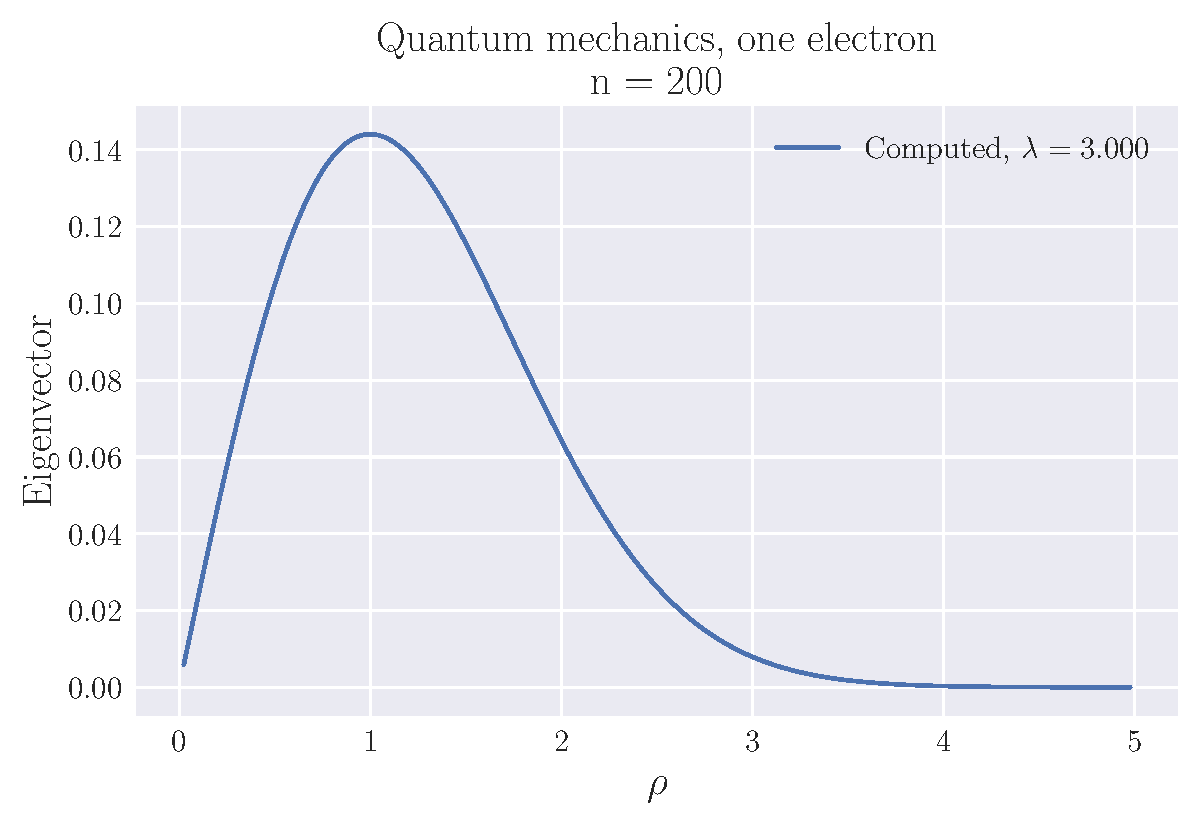
\includegraphics[width=\linewidth]{../output/QM1_200_0.pdf}
	\caption{In this figure you see the eigenvector/eigenstate for one particle in a HO potential corresponding to the smallest eigenvalue $\lambda_1$, i.e the lowest energy value. Along the x-axis we have dimensionless length $\rho$ and along the y-axis we have the elements of the eigenvector scaled to unit length. In the label we have the corresponding eigenvalue $\lambda_1 = 3.000$. The number of integration points is $n = 200$.}
  \label{fig:QM200}
\end{figure}

The result for two particles can be seen in figure \ref{fig:QM2002}. Again we tested for different endpoints and integration points, and found that $n=200$ and $\lambda_N = 5$ worked well. The reason we have not included the other plots is because they are indistinguishable to the human eye. We tested for different frequencies $\omega_r = 0.01, 0.5, 1, 5$ and got corresponding eigenvalues $\lambda = 0.841, 2.231, 4.058, 17.444$. Higher frequency seems to create larger eigenvalues, broader and lower peaks more to the right.

\begin{figure}[h]
	\centering
	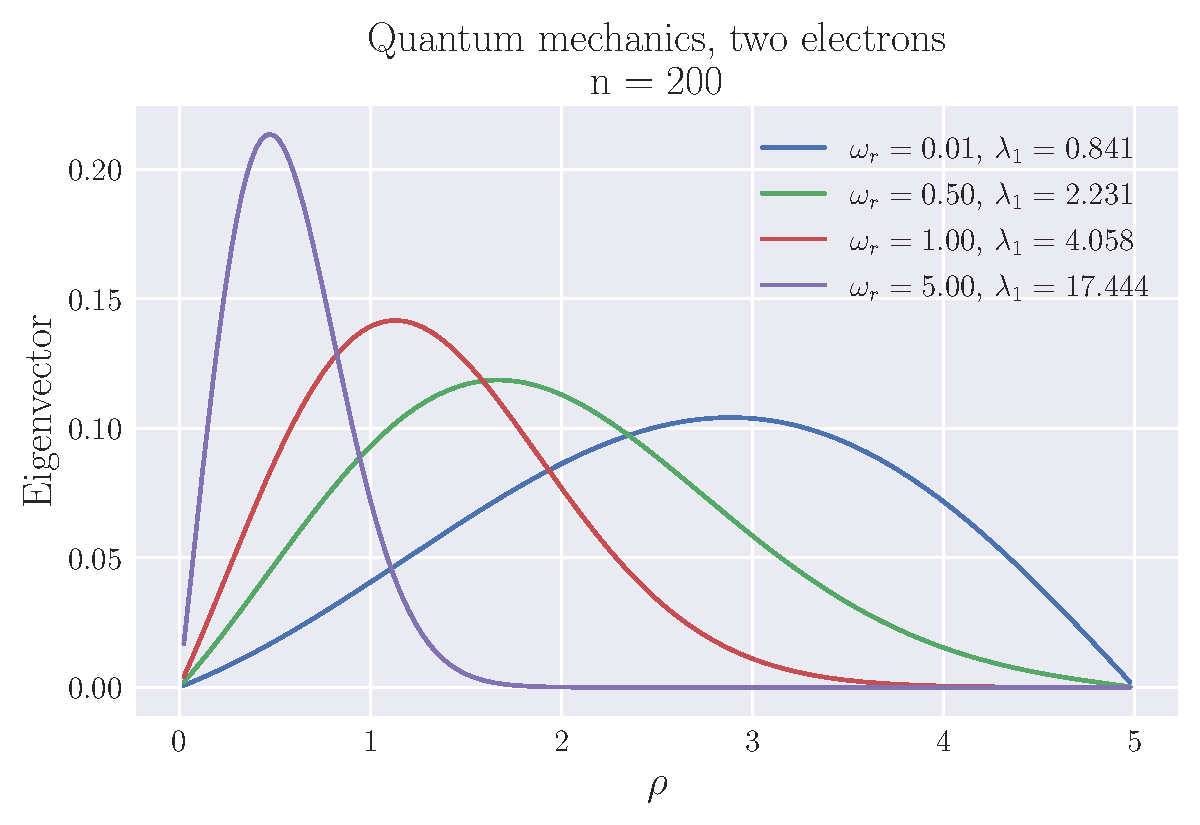
\includegraphics[width=\linewidth]{../output/QM2_200.pdf}
	\caption{The radial wave function $\psi(\rho)$ for a system of two electrons interacting through the Coulomb potential in a harmonic oscillator well. This is the function corresponding to the smallest eigenvalue $\lambda_1$, i.e the lowest energy value. The number of integration points is $n = 200$. The eigenvector is normalized to length 1.}
  \label{fig:QM2002}
\end{figure}

For those interested have we listed the numbers of iterations (see table \ref{tab:iter}) and time needed (see table \ref{tab:time}) in order to complete the algorithm, for different integration points.

\begin{table}[h]
	\input{../output/table_iters.txt}
	\label{tab:iter}
	\caption{This table shows the total number of iterations needed for different integration points N. BB corresponds to buckling beam, QM1 one particle in HO potential and QM2 two particles.}
\end{table}

\begin{table}[h]
	\input{../output/table_time.txt}
	\label{tab:time}
	\caption{This table show the total time (in milliseconds) needed to perform the computations for different integration points N. BB corresponds to buckling beam, QM1 one particle in HO potential and QM2 two particles.}
\end{table}

\section{Discussion}

\subsection{FLOPS in Jacobi's rotation algorithm}

It is clear from tables \ref{tab:iter} and \ref{tab:time} that the number of FLOPS (equation \ref{eq:FLOPS}) was underestimated. The number of iterations turned to be approximately five times what we estimated:
\begin{equation*}
  N_{\text{iter}} = \frac{5}{2}n^2
\end{equation*}
for $n$ integration points. The number of FLOPS per iterations was clearly missing some elements. We did not include the cost of iterating through all the elements above or below the diagonal to find the indices and value of the largest element. For all elements in the upper or lower half of the matrix, this involves at least a function call or FLOP to determine the absolute value of the element and a comparison to determine if it is greater than the largest number found so far. Though this is not an expensive operation for each element, the total number of FLOPS for all the elements combined would probably grow as $n^2$ as the number of elements grows as $n^2$. With a number of iterations that grows as $n^2$ this would result in a term in the total number of FLOPS that grows like $n^4$ which could have a substantial effect on computing time for large $n$.

\subsection{Interpretation of the results}

The tests and eigenvalue for one particle worked as expected, making us more confident that the algorithm is producing trustworthy results. For two particles we got that, for higher frequencies, we got larger eigenvalues. Since the eigenvalue corresponds to energy, that should mean we have more of it. Now the eigenvectors plotted in figure \ref{fig:QM2002} are harder to interpret. Higher frequencies leads to a more narrow peak located more to the left (lower $\rho$). In quantum mechanics a narrow graph often means that a value is more sharp, in this case $\rho$. Now $\rho$ is a representation of the relative position $r = |\mathbf{r}_1 - \mathbf{r}_2|$, where $\mathbf{r}_1$ and $\mathbf{r}_2$ are the positions specific particles. If we had a many, this could represent some sort of charge density, meaning that for lower $\omega_r$ it is less grouped. In other words the charge could is more diffuse and further away from the core. 

\section{Conclusion}

We used Jacobi's rotation algorithm to solve a quantum mechanical eigenvalue/vector problem. Before we applied the algorithm we did tests on an analytical system (buckling beam). We also tested the algorithm using unit-tests to test specific chunks of the program. Although we predicted a lot fewer FLOPS, the tests passed and are described with solutions in the appendix \ref{appendix}.

For one particle Jacobi's rotation algorithm produces the eigenvalue $\lambda = 3.000$ for the lowest state. This is close to the analytical term of $\lambda_{ana} = 3$. For two particles we get the eigenvalues (lowest energy state) $\lambda = 0.841, 2.231, 4.058, 17.444$ with the corresponding frequencies $\omega_r = 0.01, 0.5, 1, 5$. This means that the energy gets higher with larger frequency $\omega_r$. We also notice that the eigenvector plotted, is wider, lower and more to the right (higher $\rho$) for lower frequencies. The fact that the graph is wider might mean $\rho$ is less sharp, telling us that maybe the charge density is less grouped together for lower frequencies. Our physical interpretation of the maximum being more to the right $\omega_r$ corresponds to a orbit further away from the core. If $\omega_r$ also represents the speed of which the particles orbit, it also makes sense that the orbit becomes smaller.

\section{Appendix}
\label{appendix}

\subsection{Buckling beam}

The simplest use case for our algorithm is a second order differential equation like \ref{eq:SE1} and \ref{eq:SE2}, but without the potential. One such example is equation \ref{eq:BB} for the vertical displacement $u(\rho)$ of a horisontal beam of length $L$ when a force is applied in the x-direction towards the origin. $\rho = x/L \in [0, 1]$, where $L$ is the length of the beam, is a dimensionless length. The constant $\lambda$ can be expressed as $\lambda = F L^2 / \gamma$, where $F$ is the applied force and $\gamma$ is a constant defined by properties like the rigidity of the beam.
\begin{equation}
	-\frac{d^2}{d\rho^2}u(\rho) = \lambda u(\rho)
	\label{eq:BB}
\end{equation}

Discretizing this equation gives a matrix equation on the form of equation \ref{eq:discrete_2nd_deriv_mat} with $e_i = e = -1/h^2$ and $d_i = d = 2/h^2$, where $h$ again is the step size. This is a tridiagonal Toeplitz matrix which has analytical eigenvalues described by \ref{eq:BB_eigvals} and analytical eigenvectors described by \ref{eq:BB_eigvecs}, both for $j = 1, 2, ..., N-1$. Figure \ref{fig:BB200} shows the eigenvector corresponding to the smallest eigenvalue, both computed and analytic, for $n = 200$ integration points.
\begin{align}
  \lambda_j &= d + 2 e \cos{\left( \frac{j \pi}{N} \right)} \label{eq:BB_eigvals} \\
  \mathbf u_j &= \left[ \sin{\left( \frac{j \pi}{N} \right)}, \sin{\left( \frac{2 j \pi}{N} \right)}, ..., \sin{\left( \frac{(N-1) j \pi}{N} \right)} \right]^T \label{eq:BB_eigvecs}
\end{align}

\begin{figure}[h]
	\centering
	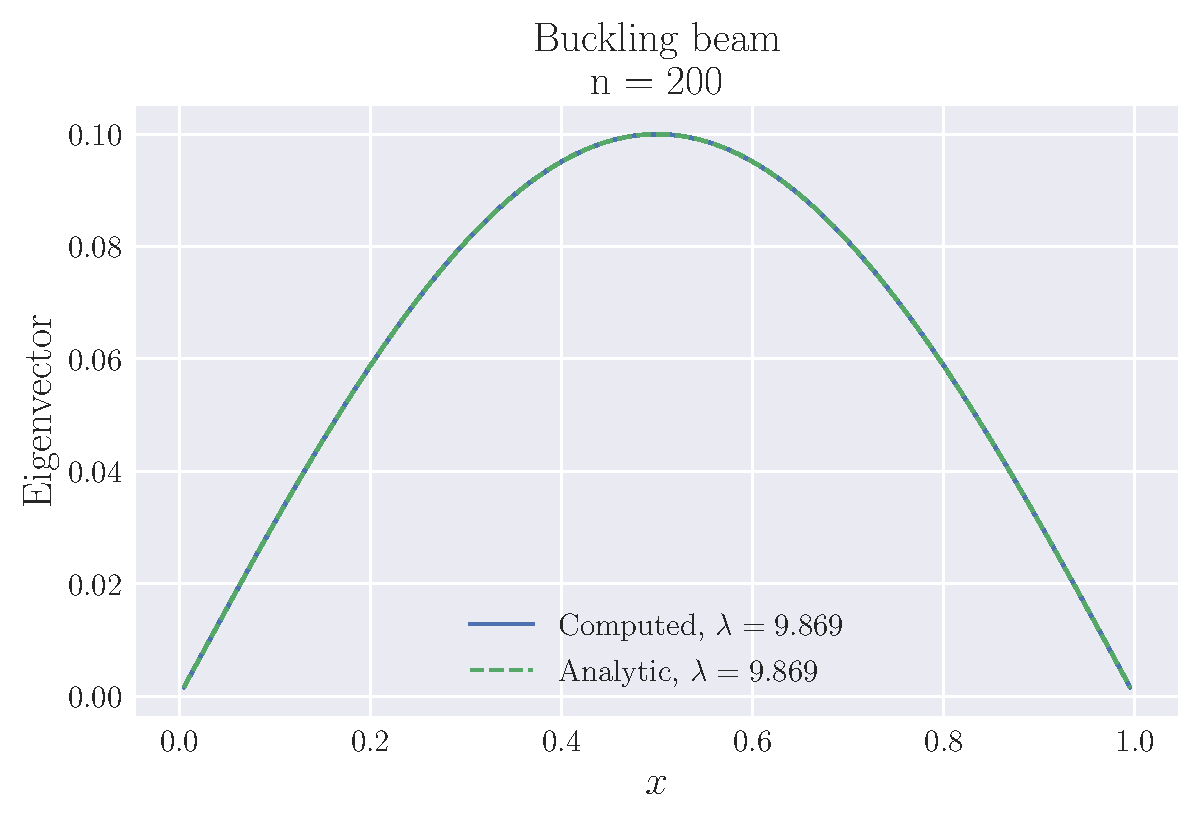
\includegraphics[width=\linewidth]{../output/BB_200_0.pdf}
	\caption{The displacement $u(\rho)$ of a buckling beam corresponding to the smallest eigenvalue $\lambda_1$. The number of integration points is $n = 200$. The eigenvector is normalized to length 1.}
  \label{fig:BB200}
\end{figure}


\subsection{Unit-tests}

There are several sections in this code that can be tested independently. We have developed tests for a general tridiagonal Toeplitz matrix that checks that the program finds the correct indices $k$ and $l$ for the largest off-diagonal element in the matrix and that the computed eigenvalues and eigenvectors match the analytic results in equations \ref{eq:BB_eigvals} and \ref{eq:BB_eigvecs}. For $n = 10$, the tests pass with a tolerance of $10^{-3}$ for the eigenvalues and $10^{-2}$ for each element in the eigenvector corresponding to the smallest eigenvalue. Figure \ref{fig:BB200} displaying the results of the algorithm does indeed show a very good correspondence between computed and analytic results.


\onecolumngrid
\begin{thebibliography}{}
\bibitem{lecnotes} Computational Physics I FYS3150/FYS4150, Department of Physics, Univeristy of Oslo, Sep 30, 2020, http://compphysics.github.io/
ComputationalPhysics/doc/pub/eigvalues/html/.\_eigvalues-bs011.html
\bibitem{oppgavetekst} Project 2, Computational Physics I FYS3150/FYS4150, Department of Physics, Univeristy of Oslo, Sep 11, 2020.

\end{thebibliography}
\end{document}
